%  LaTeX support: latex@mdpi.com
%  In case you need support, please attach all files that are necessary for compiling as well as the log file, and specify the details of your LaTeX setup (which operating system and LaTeX version / tools you are using).

%=================================================================
\documentclass[water,article,submit,moreauthors,pdftex]{mdpi}

% If you would like to post an early version of this manuscript as a preprint, you may use preprint as the journal and change 'submit' to 'accept'. The document class line would be, e.g., \documentclass[preprints,article,accept,moreauthors,pdftex]{mdpi}. This is especially recommended for submission to arXiv, where line numbers should be removed before posting. For preprints.org, the editorial staff will make this change immediately prior to posting.

%% Some pieces required from the pandoc template
\providecommand{\tightlist}{%
  \setlength{\itemsep}{0pt}\setlength{\parskip}{4pt}}
\setlist[itemize]{leftmargin=*,labelsep=5.8mm}
\setlist[enumerate]{leftmargin=*,labelsep=4.9mm}

\usepackage{longtable}

% see https://stackoverflow.com/a/47122900

%--------------------
% Class Options:
%--------------------
%----------
% journal
%----------
% Choose between the following MDPI journals:
% acoustics, actuators, addictions, admsci, aerospace, agriculture, agriengineering, agronomy, algorithms, animals, antibiotics, antibodies, antioxidants, applsci, arts, asc, asi, atmosphere, atoms, axioms, batteries, bdcc, behavsci , beverages, bioengineering, biology, biomedicines, biomimetics, biomolecules, biosensors, brainsci , buildings, cancers, carbon , catalysts, cells, ceramics, challenges, chemengineering, chemistry, chemosensors, children, cleantechnol, climate, clockssleep, cmd, coatings, colloids, computation, computers, condensedmatter, cosmetics, cryptography, crystals, dairy, data, dentistry, designs , diagnostics, diseases, diversity, drones, econometrics, economies, education, electrochem, electronics, energies, entropy, environments, epigenomes, est, fermentation, fibers, fire, fishes, fluids, foods, forecasting, forests, fractalfract, futureinternet, futurephys, galaxies, games, gastrointestdisord, gels, genealogy, genes, geohazards, geosciences, geriatrics, hazardousmatters, healthcare, heritage, highthroughput, horticulturae, humanities, hydrology, ijerph, ijfs, ijgi, ijms, ijns, ijtpp, informatics, information, infrastructures, inorganics, insects, instruments, inventions, iot, j, jcdd, jcm, jcp, jcs, jdb, jfb, jfmk, jimaging, jintelligence, jlpea, jmmp, jmse, jnt, jof, joitmc, jpm, jrfm, jsan, land, languages, laws, life, literature, logistics, lubricants, machines, magnetochemistry, make, marinedrugs, materials, mathematics, mca, medicina, medicines, medsci, membranes, metabolites, metals, microarrays, micromachines, microorganisms, minerals, modelling, molbank, molecules, mps, mti, nanomaterials, ncrna, neuroglia, nitrogen, notspecified, nutrients, ohbm, particles, pathogens, pharmaceuticals, pharmaceutics, pharmacy, philosophies, photonics, physics, plants, plasma, polymers, polysaccharides, preprints , proceedings, processes, proteomes, psych, publications, quantumrep, quaternary, qubs, reactions, recycling, religions, remotesensing, reports, resources, risks, robotics, safety, sci, scipharm, sensors, separations, sexes, signals, sinusitis, smartcities, sna, societies, socsci, soilsystems, sports, standards, stats, surfaces, surgeries, sustainability, symmetry, systems, technologies, test, toxics, toxins, tropicalmed, universe, urbansci, vaccines, vehicles, vetsci, vibration, viruses, vision, water, wem, wevj

%---------
% article
%---------
% The default type of manuscript is "article", but can be replaced by:
% abstract, addendum, article, benchmark, book, bookreview, briefreport, casereport, changes, comment, commentary, communication, conceptpaper, conferenceproceedings, correction, conferencereport, expressionofconcern, extendedabstract, meetingreport, creative, datadescriptor, discussion, editorial, essay, erratum, hypothesis, interestingimages, letter, meetingreport, newbookreceived, obituary, opinion, projectreport, reply, retraction, review, perspective, protocol, shortnote, supfile, technicalnote, viewpoint
% supfile = supplementary materials

%----------
% submit
%----------
% The class option "submit" will be changed to "accept" by the Editorial Office when the paper is accepted. This will only make changes to the frontpage (e.g., the logo of the journal will get visible), the headings, and the copyright information. Also, line numbering will be removed. Journal info and pagination for accepted papers will also be assigned by the Editorial Office.

%------------------
% moreauthors
%------------------
% If there is only one author the class option oneauthor should be used. Otherwise use the class option moreauthors.

%---------
% pdftex
%---------
% The option pdftex is for use with pdfLaTeX. If eps figures are used, remove the option pdftex and use LaTeX and dvi2pdf.

%=================================================================
\firstpage{1}
\makeatletter
\setcounter{page}{\@firstpage}
\makeatother
\pubvolume{xx}
\issuenum{1}
\articlenumber{5}
\pubyear{2019}
\copyrightyear{2019}
%\externaleditor{Academic Editor: name}
\history{Received: date; Accepted: date; Published: date}
\updates{yes} % If there is an update available, un-comment this line

%% MDPI internal command: uncomment if new journal that already uses continuous page numbers
%\continuouspages{yes}

%------------------------------------------------------------------
% The following line should be uncommented if the LaTeX file is uploaded to arXiv.org
%\pdfoutput=1

%=================================================================
% Add packages and commands here. The following packages are loaded in our class file: fontenc, calc, indentfirst, fancyhdr, graphicx, lastpage, ifthen, lineno, float, amsmath, setspace, enumitem, mathpazo, booktabs, titlesec, etoolbox, amsthm, hyphenat, natbib, hyperref, footmisc, geometry, caption, url, mdframed, tabto, soul, multirow, microtype, tikz

%=================================================================
%% Please use the following mathematics environments: Theorem, Lemma, Corollary, Proposition, Characterization, Property, Problem, Example, ExamplesandDefinitions, Hypothesis, Remark, Definition
%% For proofs, please use the proof environment (the amsthm package is loaded by the MDPI class).

%=================================================================
% Full title of the paper (Capitalized)
\Title{Data Collection in the US: Policy Recommendations for Protecting
Individuals' Privacy}

% Authors, for the paper (add full first names)
\Author{Audrey Bertin$^{1}$}

% Authors, for metadata in PDF
\AuthorNames{Audrey Bertin}

% Affiliations / Addresses (Add [1] after \address if there is only one affiliation.)
\address{%
$^{1}$ \quad Smith College - Department of Statistical and Data Sciences
Northampton, MA, USA; \\
}
% Contact information of the corresponding author
\corres{Correspondence: }

% Current address and/or shared authorship








% The commands \thirdnote{} till \eighthnote{} are available for further notes

% Simple summary

% Abstract (Do not insert blank lines, i.e. \\)
\abstract{The US is currently facing challenges with data privacy. In
the modern age, the personal information of millions of Americans is
collected and tracked daily. Data has essentially become a currency,
with companies putting ethics aside to try and collect as much
data---and therefore as much profit---as possible, threatening
individuals' rights to privacy and placing them at risk of harm. Unlike
many other developed countries, the US has taken little action at the
national level to address this issue. We consider why that is and
propose recommendations for how the US can proceed to address the issue
through policy.}

% Keywords

% The fields PACS, MSC, and JEL may be left empty or commented out if not applicable
%\PACS{J0101}
%\MSC{}
%\JEL{}

%%%%%%%%%%%%%%%%%%%%%%%%%%%%%%%%%%%%%%%%%%
% Only for the journal Diversity
%\LSID{\url{http://}}

%%%%%%%%%%%%%%%%%%%%%%%%%%%%%%%%%%%%%%%%%%
% Only for the journal Applied Sciences:
%\featuredapplication{Authors are encouraged to provide a concise description of the specific application or a potential application of the work. This section is not mandatory.}
%%%%%%%%%%%%%%%%%%%%%%%%%%%%%%%%%%%%%%%%%%

%%%%%%%%%%%%%%%%%%%%%%%%%%%%%%%%%%%%%%%%%%
% Only for the journal Data:
%\dataset{DOI number or link to the deposited data set in cases where the data set is published or set to be published separately. If the data set is submitted and will be published as a supplement to this paper in the journal Data, this field will be filled by the editors of the journal. In this case, please make sure to submit the data set as a supplement when entering your manuscript into our manuscript editorial system.}

%\datasetlicense{license under which the data set is made available (CC0, CC-BY, CC-BY-SA, CC-BY-NC, etc.)}

%%%%%%%%%%%%%%%%%%%%%%%%%%%%%%%%%%%%%%%%%%
% Only for the journal Toxins
%\keycontribution{The breakthroughs or highlights of the manuscript. Authors can write one or two sentences to describe the most important part of the paper.}

%\setcounter{secnumdepth}{4}
%%%%%%%%%%%%%%%%%%%%%%%%%%%%%%%%%%%%%%%%%%

% Pandoc citation processing

\usepackage{float} \floatplacement{figure}{H}

\begin{document}
%%%%%%%%%%%%%%%%%%%%%%%%%%%%%%%%%%%%%%%%%%

The United States is currently facing a crisis of personal data privacy.
In recent decades, a new era in the digital world---commonly termed the
\emph{Internet of Things}, or IoT---has emerged. The IoT refers to the
technologies, devices, and people who enable the sharing of data
worldwide, and is used to characterize the modern internet age as one
whose focus is now on big data (\citet{atzori2010internet},
\citet{elvy2018commodifying}).

Improvements in computing power and internet speed, alongside the
development of new technologies capable of storing and utilizing massive
quantities of data, have ushered in a new economic age: the data
economy. Data is now a hot commodity, with the power to be incredibly
valuable to those with the technology to utilize them. According to the
big data strategist at Oracle, a major software company, ``data is in
fact a new kind of capital on par with financial capital for creating
new products and services'' (\citet{oracle_quote}). Data provides this
value through several means: by enabling businesses to profile and
target people, leading to higher success rates in attracting customers;
by providing information that can be used to help optimize systems; by
helping manage and control things; by allowing companies to model
probabilities more accurately; and by allowing certain software to
operate in a way that would not be possible otherwise
(\citet{sadowski2019data}).

Much of this data comes directly from the general public: the people who
use the goods and services produced by companies---like Amazon, Google,
and Facebook---that participate in the data economy. These corporations
collect user data constantly and on a massive scale. Amazon tracks
users' purchases and voice commands---even going so far as to track the
lines highlighted in books bought by Kindle readers
(\citet{amazon-kindle}). Google tracks every search users make, every
YouTube video they watch, their full calendar schedule, their Gmail
messages, everywhere they go, how long they stay there, and what route
they take---even if users do not have Google Maps open
(\citet{google-safety}).

This large-scale data collection poses significant ethical implications
when considering the potential effects on consumers. For one, there is
the concern of data breeches. Since user data is collected and shared
over the internet, it is at risk of being released---or taken for
nefarious purposes---through cyber-hacking events. In 2019, hundreds of
millions of facebook users' phone numbers, locations, and emails were
stolen (\citet{fb-breach}). Facebook is not alone; many other companies
have seen serious data breaches in recent years: Yahoo, Experian,
Twitter, and Microsoft, to name a few (\citet{breaches-history}). This
danger is heightened further in situations involving private health or
financial data, leaving consumers at risk of negative impacts from the
release of sensitive health information, as well as possible identity
theft and financial harm. Additionally, the misuse or unwanted release
of information on polarizing issues such as religion, sexual
orientation, or gender identity could potentially put vulnerable
consumers in harms' way---making them targets for attack.

Even if data is not released in a breech, its use and collection can
still harm consumers in other ways. Large scale data collection is often
used to power machine learning algorithms, which use data to make
predictions about people. These algorithms---though seemingly objective
at first glance---are often negatively biased toward minoritized
individuals, described in the book \emph{Data Feminism} as those who are
``actively devalued and oppressed by a dominant group,'' often including
women, people of color, and the poor (\citet{d2020data}). For example,
facial recognition algorithms built in large part off of Facebook photos
misidentify black women at a significantly higher rate than other groups
(\citet{buolamwini2018gender}). The more data that is collected, the
more algorithms that can be created---placing minoritized individuals at
risk for potential harm due to algorithmic bias.

Data can also be used for psychological manipulation. Sites like
Facebook and Twitter have a wealth of data on their users---enough to
predict with high accuracy how they will react when exposed to certain
stimuli. These sites can use that knowledge to spread targeted messages
and actively change the beliefs held the public. This is what happened
in the 2016 election, when Facebook's advertising system targeted those
individuals it calculated to be likely susceptible to conservative
messaging with advertisements that reflected the ideals of Donald Trump.
Though not known for certain, it is widely believed that these
advertisements may have convinced enough voters to support President
Trump that he eventually won the election (\citet{fb-election}).

The practice of mass data collection is far from ethically sound. In
spirit---though not officially declared by law on the federal level---it
violates one of the founding principles of the United States:
individuals' right to privacy. The right to privacy is a crucial
foundation of this country. It was first officially alluded to in the
Fourth Amendment to the constitution---though it is implied to some
degree in the First, Third, and Fifth as well---and has been reinforced
at the highest levels of the judicial system for centuries.

Mass data collection can also put individuals' First and Fourteenth
Amendment rights at risk. Freedom of speech and of expression are
threatened by the possibility of data breeches---users who fear that
their data may be taken and used by unauthorized individuals may refrain
from sharing controversial opinions or personal information on religion,
sexual orientation, or other sensitive matters online, for fear that it
may be used against them when they would have otherwise done so if not
fearful of an information breach. The equal protection clause of the
Fourteenth Amendment is likewise threatened. Although not necessary
intentional, the bias present in the mass public/consumer data
algorithms has the effect of treating equal groups differently,
which---if used in certain circumstances---can violate the principle
that all people deserve equal protection.

Now, more than ever, Americans have lost faith in the ability of
companies to protect their private data, and their trust only lessens
year by year (\citet{olmstead2017americans}).

Despite all of the dangers and ethical concerns inherent in mass data
collection, companies still continue to practice it because of the
financial benefits. Lawmakers in the United States have recognized the
problem and attempted to solve it through legislation, but their efforts
have fallen short. The US has failed to produce any comprehensive
legislation on data privacy at the federal level and at the state level
there exists only a patchwork of laws, plagued by inconsistencies,
conflicting information, and sub-optimal enforcement procedures
(\citet{cfr-reform}).

Healthcare data is by far the most protected variety, though even it
lacks a clear and comprehensive piece of legislation. The Health
Insurance Portability and Accountability Act (HIPAA) only applies to
certain ``covered entities,'' and does not protect people in all
situations (\citet{hipaa}). Student health records are covered under a
different law, the Family Educational Rights and Privacy Act, which
occasionally combines or conflicts with the Children's Online Protection
Privacy Act (COPPA), meant only to protect the data of children under 13
years of age (\citet{ferpa-coppa}, \citet{cfr-reform}).

This failure to protect personal data is unique in the industrialized
world. 128 countries out of 194 worldwide have put in place national
data protection laws, many of which are quite strict and offer citizens
significant control over the use of their data (\citet{unctad}).

Citizens of the European Union (EU) are protected under the Global Data
Protection Regulation (GDPR), a comprehensive piece of data privacy
legislation which gives individuals in the EU the power to control what
data is collected on them and what is done with it in addition to
restricting the transfer of personal data from EU members to other
countries. The GDPR is relatively expansive, providing consumers with a
wide variety of privacy protections, including requirements that
individuals be quickly notified in the event of a data breach and
that---at a minimum---identifiable data must be pseudonymised.
Additionally, EU citizens are given rights to access and control their
data. Under GDPR, individuals have the right to access information about
what is being collected of them, the right to rectify mistakes, the
right to have their data erased or to restrict/object to processing, as
well as rights related to automated decision making and profiling.
Companies (data ``controllers'') are required to meet high privacy
standards, and there are systems in place to ensure compliance. These
include Data Protection Officers, appointed to help observe and promote
compliance, alongside a tiered fine system for GDPR violations
(\citet{GDPR-text}).

The EU is not the only region in the world that has strong data
protection laws. South Korea, for example, has the Personal Information
Protection Act (PIPA). This law is very similar to the GDPR, with
requirements for at least pseudonymising the data. PIPA also contains
rules for measures that must be taken when handling personal data to
ensure privacy. Express consent is required for the collection of
personal data, with a specific focus on sensitive data. Information such
as passport or drivers license number and information about ideology,
religion, health, sexual orientation, or other sensitive subjects must
be collected separately from one another \emph{and} separately from any
other consent. Citizens also possess similar rights to under the GDPR,
including access, correction, suspension of use, and removal of personal
data (\citet{data-guidance}).

Some countries have even gone so far as to declare data privacy a
fundamental right. In Chile, the official constitution (Article 19,
Number 4) establishes the individuals right to (i) respect and
protection of private life, (ii) honor of the person and his/her family,
and (iii) \textbf{protection of his/her personal data}. Anyone whose
rights are threatened or disturbed has the power to file a
Constitutional Protective Action in response (\citet{chile}).

Despite the apparent constitutional focus on privacy in the country, it
is clear that the United States trails far behind other developed
countries in terms of data privacy protections. Why is this?

Perhaps the most important factor in preventing nationwide data privacy
regulation is the role of the technology lobby in politics. Many of the
world's most powerful technology companies are headquartered in the
United States: Facebook, Google, Microsoft, Twitter, and Oracle, to name
a few. Bringing in hundreds of billions of dollars in revenue, these
companies play a pivotal role in the US economy, and as a result they
have a lot of political power. Their large profit margins enable these
companies to lobby the US government, preventing the passing of laws and
policies that are not in their best interest financially. Alphabet Inc,
the parent company of Google, spent 21.74 million dollars trying to
affect US policy in 2018 (\citet{tech-lobby}), and Facebook spent 19.68
million in 2020. (\citet{citizen-tech}). Technology companies have now
surpassed Big Oil and Big Tobacco---the previous most powerful lobbying
groups---as the biggest spenders in US politics, and their spending is
only increasing over time (\citet{citizen-tech}). A privacy law is
counter to these companies' best interests. Additional requirements for
data security, limitations on what can be collected, and financial
punishments for non-compliance risk damaging these companies' profits,
which rely partially on large-scale data collection. Technology
companies do not want to see a privacy law passed, and have the funding
and power available to prevent any drastic changes from happening.

\begin{figure}[H]
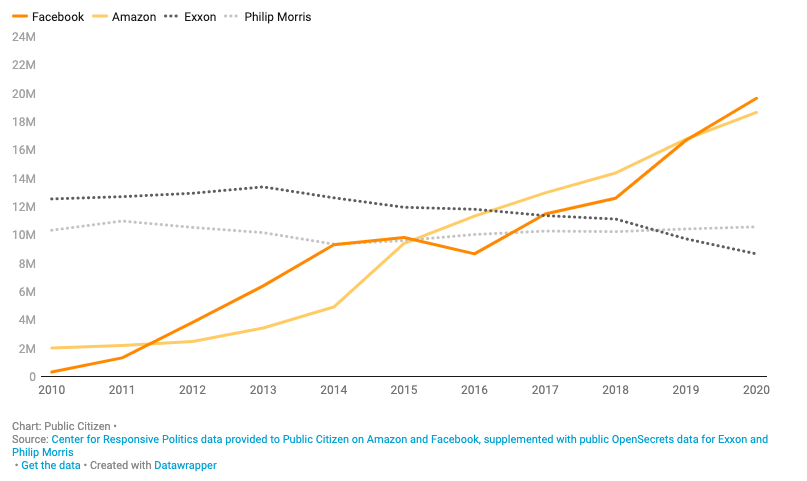
\includegraphics[width=1\linewidth]{lobby-notitle} \caption{Big Tech replaces Big Oil and Tobacco as big lobbying spenders: Total lobbying spending in Washington vs Facebook and Amazon's lobbying spending (2010-2020). Source: https://www.citizen.org/article/big-tech-lobbying-update/}\label{fig:unnamed-chunk-1}
\end{figure}

There is also the issue that the United States does not currently
possess any agency that has the ability to fully manage and ensure
compliance with a federal data privacy law. In the EU, all of the member
states have independent privacy-focused authorities to enforce the GDPR.
The US has nothing like that. The closest thing is the Federal Trade
Commission (FTC), which has historically managed other aspects of
consumer protection and privacy. However, it is relatively weak in its
powers: it is constrained in its authority, with jurisdiction primarily
in interstate commerce. The FTC can only regulate violations that meet
standards for ``unfairness and deception,'' but these are poorly defined
and unclear. Furthermore, the FTC lacks a strong record of privacy
enforcement---even in previous cases where it has had the jurisdiction
to intervene---and does not have leadership with a strong level of
technological expertise in the field of data privacy
(\citet{new-america}).

Due to the power of the technology lobby and the lack of enforcement
ability, it is difficult to imagine a large-scale, universal data
privacy law like the GPDR being passed at the national level any time in
the near future. If one were pushed in congress right now, it would
almost certainly fail, due to both challenges with its enforcement and
lobbying pressure from big tech. Instead, lawmakers wishing to institute
privacy policy will have to take a slower, step by step approach, taking
careful consideration at each step to prevent dramatic counteraction
from technology companies.

The first step necessary will likely be either the creation of a new
data protection agency or the bolstering of FTC powers to include more
oversight capability for privacy regulation. A data protection law
without an agency capable of overseeing compliance will be useless, so
this step should be completed first. As this action does not directly
and immediately financially impact technology companies, it is also one
of the more feasible policy actions available at the moment.

In the mean-time, states should continue to create their own data
privacy regulations, though with additional thought to ensure that their
proposed laws are consistent with those that have already been passed.
Although a patchwork of state laws is not optimal, the more that
individual states begin to push for privacy legislation, the more
pressure is put on the federal government to enact a policy nationwide,
as it becomes clear that the public desires change.

In the long run, however, a state-by-state patchwork will not be
sufficient and we will need a comprehensive federal law to ensure that
guidelines are consistent and all citizens are protected. The passing of
this legislation should be done with great care. Lawmakers should focus
primarily on methods for prevention of privacy failures, rather than on
mechanisms for punishment after the fact. This will ensure that the
financial harms to technology companies---in the form of large
non-compliance fines---will be minimized, making the law more palatable
to the technology lobby. Due to the significant political polarization
in United States, it is also important to ensure that any data privacy
regulations that are suggested are written in a way that is favorable to
both the Democratic and Republican parties---and, if possible, put
forward by a bipartisan coalition---so that the law is not put on hold
for political reasons. There is evidence that members of both parties
have been supportive of privacy regulation in the past
(\citet{privacy-law-bipartisan}), so this goal is not un-achievable.

The road to comprehensive data privacy legislation in the United States
is not an easy one, but it is important to uphold a standard of data
ethics and ensure that our citizens do not face dangerous outcomes from
the large-scale data collection happening in this country. Although the
US is still far behind much of the industrialized world in terms of
protecting its consumers' data privacy and many obstacles lie in the way
of changing this, with the right focus and a carefully planned course of
action, this has the potential to change for the better in the coming
years.

% %%%%%%%%%%%%%%%%%%%%%%%%%%%%%%%%%%%%%%%%%%
% %% optional
% \supplementary{The following are available online at www.mdpi.com/link, Figure S1: title, Table S1: title, Video S1: title.}
%
% % Only for the journal Methods and Protocols:
% % If you wish to submit a video article, please do so with any other supplementary material.
% % \supplementary{The following are available at www.mdpi.com/link: Figure S1: title, Table S1: title, Video S1: title. A supporting video article is available at doi: link.}

\vspace{6pt}

%%%%%%%%%%%%%%%%%%%%%%%%%%%%%%%%%%%%%%%%%%

%%%%%%%%%%%%%%%%%%%%%%%%%%%%%%%%%%%%%%%%%%

%%%%%%%%%%%%%%%%%%%%%%%%%%%%%%%%%%%%%%%%%%

%%%%%%%%%%%%%%%%%%%%%%%%%%%%%%%%%%%%%%%%%%
%% optional

\input{"appendix.tex"}

%%%%%%%%%%%%%%%%%%%%%%%%%%%%%%%%%%%%%%%%%%
% Citations and References in Supplementary files are permitted provided that they also appear in the reference list here.

%=====================================
% References, variant A: internal bibliography
%=====================================
%\reftitle{References}
%\begin{thebibliography}{999}
% Reference 1
%\bibitem[Author1(year)]{ref-journal}
%Author1, T. The title of the cited article. {\em Journal Abbreviation} {\bf 2008}, {\em 10}, 142--149.
% Reference 2
%\bibitem[Author2(year)]{ref-book}
%Author2, L. The title of the cited contribution. In {\em The Book Title}; Editor1, F., Editor2, A., Eds.; Publishing House: City, Country, 2007; pp. 32--58.
%\end{thebibliography}

% The following MDPI journals use author-date citation: Arts, Econometrics, Economies, Genealogy, Humanities, IJFS, JRFM, Laws, Religions, Risks, Social Sciences. For those journals, please follow the formatting guidelines on http://www.mdpi.com/authors/references
% To cite two works by the same author: \citeauthor{ref-journal-1a} (\citeyear{ref-journal-1a}, \citeyear{ref-journal-1b}). This produces: Whittaker (1967, 1975)
% To cite two works by the same author with specific pages: \citeauthor{ref-journal-3a} (\citeyear{ref-journal-3a}, p. 328; \citeyear{ref-journal-3b}, p.475). This produces: Wong (1999, p. 328; 2000, p. 475)

%=====================================
% References, variant B: external bibliography
%=====================================
\reftitle{References}
\externalbibliography{yes}
\bibliography{citations.bib}

%%%%%%%%%%%%%%%%%%%%%%%%%%%%%%%%%%%%%%%%%%
%% optional

%% for journal Sci
%\reviewreports{\\
%Reviewer 1 comments and authors’ response\\
%Reviewer 2 comments and authors’ response\\
%Reviewer 3 comments and authors’ response
%}

%%%%%%%%%%%%%%%%%%%%%%%%%%%%%%%%%%%%%%%%%%
\end{document}
